\documentclass[tikz]{standalone}
\usepackage{amssymb,dsfont}
\usepackage{color}
\usetikzlibrary{arrows}
% Sets
\newcommand{\CC}{\mathbb{C}}        % Complex numbers
\newcommand{\NN}{\mathbb{N}}        % Natural numbers
\newcommand{\RR}{\mathbb{R}}        % Real numbers
\newcommand{\ZZ}{\mathbb{Z}}        % Relative integers
% Groups
\newcommand{\SO}{\mathrm{SO}}       % Special orthogonal group
\newcommand{\OO}{\mathrm{O}}        % Orthogonal group
\newcommand{\SU}{\mathrm{SU}}       % Special unitary group
\newcommand{\1}{\mathds{1}}		    % trivial group
\newcommand{\DD}{\mathbb{D}}        % Dihedral group
\newcommand{\octa}{\mathbb{O}}      % Cubic (octahedral) group
\newcommand{\ico}{\mathbb{I}}       % Icosahedral group
\newcommand{\tetra}{\mathbb{T}}     % tetrahedral group
\begin{document}
	
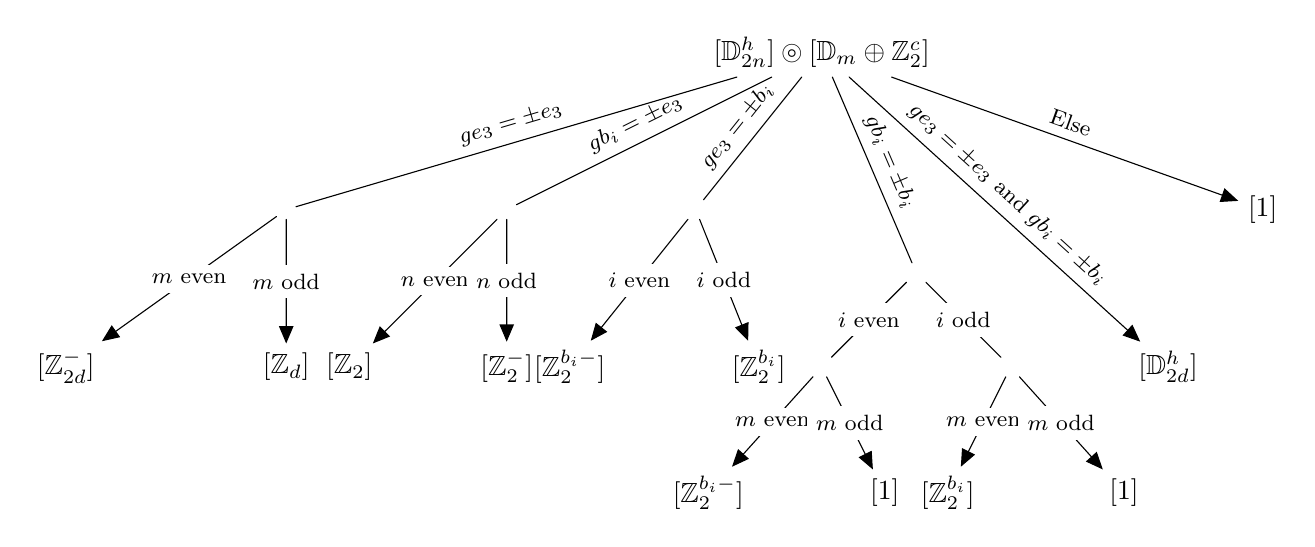
\begin{tikzpicture}[scale=0.8,line cap=round,line join=round,>=triangle 45,x=1.0cm,y=1.0cm]
  \node (root) at (0,0) {$[\DD_{2n}^h]\circledcirc [\DD_m\oplus \ZZ_2^c]$};

  \node (Bas1) at (-8.5,-2.5) {};
  \node (Bas2) at (-5,-2.5) {};
  \node (Bas3) at (-2,-2.5) {};
  \node (Bas4) at (1.5,-3.5)  {};
  \node (Bas5) at (5.5,-5)  {$[\DD_{2d}^h]$};
  \node (Bas6) at (7,-2.5) {$[\1]$};
  \draw    (root) -- (Bas1) node [midway,above,sloped] {{\footnotesize  $ge_3=\pm e_3$ }};
  \draw    (root) -- (Bas2) node [midway,above,sloped] {{\footnotesize  $gb_i=\pm e_3$}};
  \draw    (root) -- (Bas3) node [midway,above,sloped] {{\footnotesize  $ge_3=\pm b_i$}};
  \draw    (root) -- (Bas4) node [midway,above,sloped] {{\footnotesize  $gb_i=\pm b_i$}};
  \draw[->](root) -- (Bas5) node [midway,above,sloped] {{\footnotesize  $ge_3=\pm e_3$ and $gb_i=\pm b_i$}};
  \draw[->](root) -- (Bas6) node [midway,above,sloped] {{\footnotesize  Else}};
  \node (Bas11) at (-8.5-3.5,-5) {$[\ZZ_{2d}^-]$};
  \node (Bas12) at (-8.5,-5) {$[\ZZ_d]$};
  \draw[->] (Bas1) -- (Bas11) node [midway,fill=white] {{\footnotesize  $m$ even}};
  \draw[->] (Bas1) -- (Bas12) node [midway,fill=white] {{\footnotesize  $m$ odd}};
  \node (Bas21) at (-5-2.5,-5) {$[\ZZ_2]$};
  \node (Bas22) at (-5,-5) {$[\ZZ_2^-]$};
  \draw[->] (Bas2) -- (Bas21) node [midway,fill=white] {{\footnotesize  $n$ even}};
  \draw[->] (Bas2) -- (Bas22) node [midway,fill=white] {{\footnotesize  $n$ odd}};
  \node (Bas31) at (-2.5-1.5,-5) {$[\ZZ_2^{b_i-}]$};
  \node (Bas32) at (-2.5+1.5,-5)  {$[\ZZ_2^{b_i}]$};
  \draw[->] (Bas3) -- (Bas31) node [midway,fill=white] {{\footnotesize  $i$ even}};
  \draw[->] (Bas3) -- (Bas32) node [midway,fill=white] {{\footnotesize  $i$ odd}};
  \node (Bas41) at (1.5-1.5,-5) {};
  \node (Bas42) at (1.5+1.5,-5)  {};
  \draw (Bas4) -- (Bas41) node [midway,fill=white] {{\footnotesize  $i$ even}};
  \draw (Bas4) -- (Bas42) node [midway,fill=white] {{\footnotesize  $i$ odd}};
  \node (Bas411) at (1.5-1.5-1.8,-7) {$[\ZZ_2^{b_i-}]$};
  \node (Bas412) at (1.5-1.5+1,-7)  {$[\1]$};
  \draw[->] (Bas41) -- (Bas411) node [midway,fill=white] {{\footnotesize  $m$ even}};
  \draw[->] (Bas41) -- (Bas412) node [midway,fill=white] {{\footnotesize  $m$ odd}};
  \node (Bas421) at (1.5+1.5-1,-7) {$[\ZZ_2^{b_i}]$};
  \node (Bas422) at (1.5+1.5+1.8,-7)  {$[\1]$};
  \draw[->] (Bas42) -- (Bas421) node [midway,fill=white] {{\footnotesize  $m$ even}};
  \draw[->] (Bas42) -- (Bas422) node [midway,fill=white] {{\footnotesize  $m$ odd}};
\end{tikzpicture}
% Further ’tikzpicture’ environments are possible which will create further pages.
\end{document} 